\chapter{Autoregulon Networks: COMING SOON}
\label{ch-autoregulons}

This chapter is based on Ref.\cite{alon-book}.

Appendix \ref{ch-genomics-vocab}

\section{Autoregulon net motif}
a {\bf net motif} is just a subgraph of a bnet

\begin{figure}[h!]
$$
\xymatrix{
&\rvx\ar[dd]|{-\alp}\ar[dl]
\\
f(\rvx)\ar[dr]|{1}
\\
&\Circle{\frac{d\rvx}{dt}}
}\quad
\xymatrix{\\=}
\quad
\xymatrix{
\\
\rvx\ar@{=>}[d]
\\
\dot{\rvx}
}
$$
\caption{Autoregulon net motif and the symbol we will
use to denote it when we consider
networks of connected autoregulons. Assume $\alp >0$.}
\label{fig-net-motif}
\end{figure}

\beq
\frac{dx}{dt}=f(x)-\alp x
\eeq

\beq
f(x)=\left\{
\begin{array}{ll}
\beta\indi(x<K)
&(f \text{ is lowpass})
\\
\beta\indi(x>K)
&(f \text{ is highpass})
\end{array}
\right.
\eeq
where $\alp, \beta > 0$.

Lowpass $f$ describes a {\bf repressor}.
Highpass $f$ describes an activator.

\hrule
For $f$ lowpass
\beq
x= 
\left\{
\begin{array}{ll}
x_0 e^{-\alp t} +
\frac{\beta}{\alp}\left[1-e^{-\alp t}\right]
&\text{ if } t<t_K
\\
x_K e^{-\alp (t-t_K)}
&\text{ if } t>t_K
\end{array}
\right.
\eeq
where, to make $x(t)$ continuous at $t=t_K$ and $x(t_K)=x_K$,
we must have

\beq
 x_0 e^{-\alp t_K} +
\frac{\beta}{\alp}
\left[1-e^{-\alp t_K}\right]
=
x_K
\eeq

Note that if $\alp t<<1$, then\footnote{Use $e^x\approx 1 + x$ for $|x|<<1$.}, 

\beqa
x &\approx&
x_0(1-\alp t) +\beta t
\\ &=&
x_0 + (\beta -\alp x_0)t
\eeqa

Assume $x_0=0$ for simplicity.
In that case, if $K>\frac{\beta} {\alp}$, $t_K$ 
doesn't exist and only the $t<t_K$
branch of the $x$ solution above exists.
On the other hand, if $K<\frac{\beta} {\alp}$, 
then $t_K$ exists and $x_K=K$.
For $t>t_K$,

\beq
x=
K e^{-\alp(t-t_K)}
\eeq

\begin{figure}[h!]
\centering
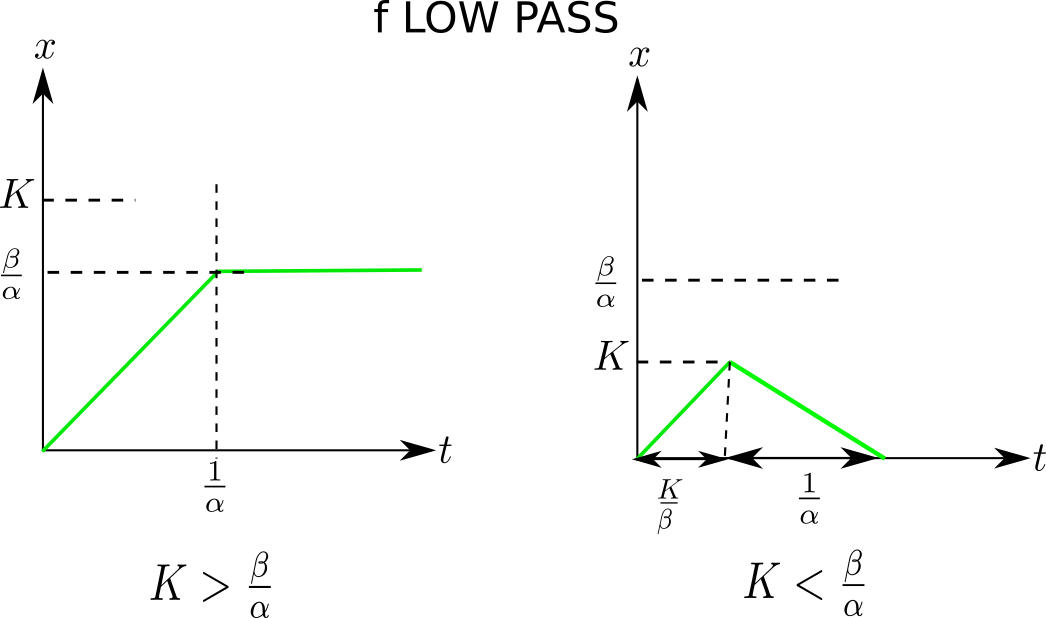
\includegraphics[width=4in]
{autoregulons/autoreg-lowpass.png}
\caption{Approximate $x$ for autoregulon with lowpass $f$
and $x_0=0$}
\label{fig-autoreg-lowpass}
\end{figure}

See Fig.\ref{fig-autoreg-lowpass}
for approximate 
$x$ for autoregulon with lowpass $f$
and $x_0=0$.


\hrule
For $f$ highpass

\beq
x= 
\left\{
\begin{array}{ll}
x_0 e^{-\alp t} &\text{ if } t<t_K  
\\
x_K e^{-\alp (t-t_K)} +
\frac{\beta}{\alp}
\left[ 1-e^{-\alp (t-t_K)}\right]
&\text{ if } t>t_K
\end{array}
\right.
\eeq
where, to make $x(t)$ continuous at $t=t_K$ and $x(t_K)=x_K$,
we must have

\beq
x_0 e^{-\alp t_K} = x_K
\eeq

Note that if $\alp t<<1$, then

\beqa
x &\approx&
x_0(1 -\alp t)
\eeqa
Unlike when $f$ is lowpass, 
in this case of $f$ highpass,
we can't assume $x_0=0$ or else $x_K=K=0$ too. In fact, we must have $x_0 > x_K=K$. For $\alp (t-t_K) >>1$, 
\beq
x\approx \frac{\beta}{\alp}
\eeq

\begin{figure}[h!]
\centering
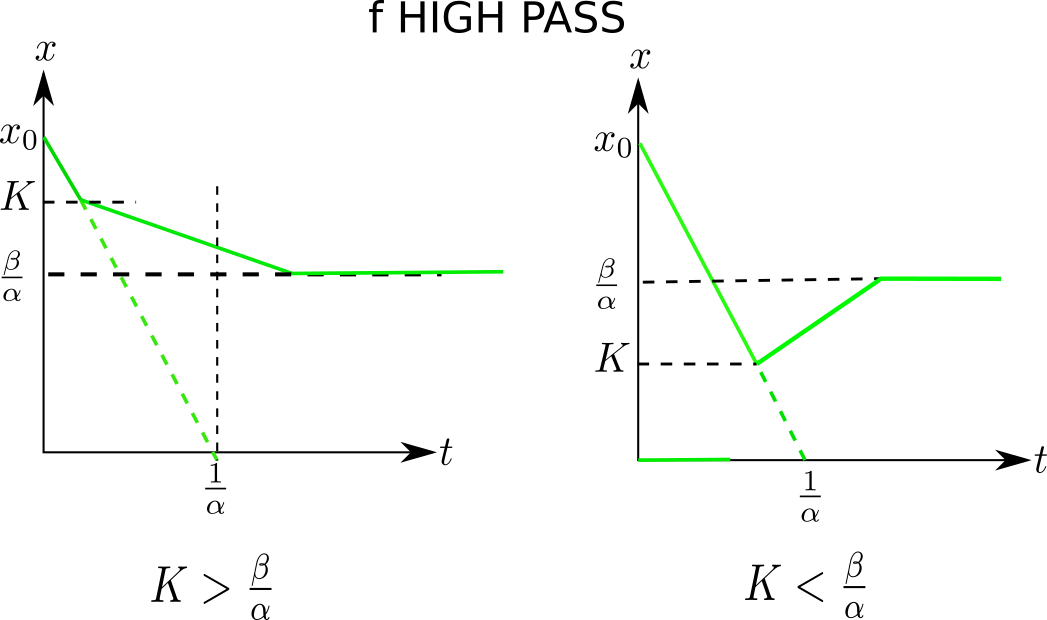
\includegraphics[width=4in]
{autoregulons/autoreg-highpass.png}
\caption{Approximate $x$ for autoregulon with highpass $f$}
\label{fig-autoreg-highpass}
\end{figure}
See Fig.\ref{fig-autoreg-highpass}
for picture of 
approximate $x$ for autoregulon with highpass $f$.

\hrule


Three $x$ values $\{x_0, K, \frac{\beta}{\alp}\}$, and
two $f$ values $\{ \text{lowpass, highpass}\}$






\section{Multiple autoregulons}




\begin{figure}[h!]
$$
\xymatrix@C=6pc@R=1pc{
\rvx \ar@{=>}[dd]\ar[ddr]|<<<<{\gamma_{\rvy|\rvx}}
& \rvy \ar@{=>}[dd]\ar[ddl]|<<<<{\gamma_{\rvx|\rvy}}
\\
&
\\
\dot{\rvx}
&\dot{\rvy}
}
\xymatrix{\\
\quad=\quad}
\xymatrix@C=5pc{
\\
\Rect{\rvx}
\autoar{r}
{\gamma_{\rvy|\rvx}}
{\gamma_{\rvx|\rvy}}
&
\Rect{\rvy}}
$$
\caption{Two autoregulons connected to each other.}
\label{fig-2-autoregulons}
\end{figure}



\beq
\left\{
\begin{array}{l}
\cald\rvx = f_\rvx(x) + \gamma_{\rvx|\rvy}\;y
\\
\cald\rvy = f_\rvy(y) +\gamma_{\rvy|\rvx}\;x
\end{array}
\right.
\eeq


\begin{figure}[h!]
$$
\xymatrix@C=4pc@R=5pc{
&\Rect{\rvx}
\autoar{ld}{}{}
\autoar{rd}{}{}
\\
\Rect{\rvy}\autoar{rr}{}{}
&&
\Rect{\rvz}
}
$$
\caption{Three autoregulons connected to each other.
$\gamma_{\rvx|\rvy}$ coefficients are left implicit.}
\label{fig-3-autoregulons}
\end{figure}



\beq
\left\{
\begin{array}{l}
\cald\rvx = f_\rvx(x)+
\gamma_{\rvx|\rvy}\;y
+
\gamma_{\rvx|\rvz}\;z
\\
\cald\rvy = f_\rvy(y)+
\gamma_{\rvy|\rvx}\;x
+
\gamma_{\rvy|\rvz}\;\rvz
\\
\cald\rvz = f_\rvz(z) +
\gamma_{\rvz|\rvx}\;x
+
\gamma_{\rvz|\rvy}\;y
\end{array}
\right.
\eeq

Use $\xymatrix{\rvx\ar[r]|{\color{red}\;+\;}&\rvy}$
to denote
$\xymatrix{\rvx\ar[r]^\alp&\rvy}$
with $\alp>0$.

Use $\xymatrix{\rvx\ar[r]|{\color{red}\;-\;}&\rvy}$
to denote
$\xymatrix{\rvx\ar[r]^\alp&\rvy}$
with $\alp<0$

Use $\xymatrix{\rvx\ar[r]|{\color{red}\;0\;}&\rvy}$
to denote
$\xymatrix{\rvx\ar[r]^\alp&\rvy}$
with $\alp=0$.

\begin{figure}[h!]
$$
\begin{array}{ccc}
\xymatrix@C=4pc@R=5pc{
&\Rect{\rvx}
\autoar{ld}{-}{0}
\autoar{rd}{+}{0}
\\
\Rect{\rvy}\autoar{rr}{-}{0}
&&
\Rect{\rvz}
}
&&
\xymatrix@C=4pc@R=5pc{
&\Rect{\rvx}
\autoar{ld}{-}{0}
\autoar{rd}{+}{0}
\\
\Rect{\rvy}\autoar{rr}{+}{0}
&&
\Rect{\rvz}
}
\\
\\
(a)&&(b)
\end{array}
$$
\caption{$(a)$ shows a coherent net of 3 autoregulons because $\sign(\gamma_{\rvz|\rvy}\gamma_{\rvy|\rvx})=\sign(\gamma_{\rvz|\rvx})$.
$(b)$ shows a incoherent net of 3 autoregulons because $\sign(\gamma_{\rvz|\rvy}\gamma_{\rvy|\rvx})\neq \sign(\gamma_{\rvz|\rvx})$.
}
\label{fig-3-coherent-autoregulons}
\end{figure}


\begin{figure}[h!]
$$
\xymatrix@C=6pc@R=2pc{
\rvx \ar@{=>}[dd]\ar[ddrr]|<<<<{\gamma_{\rvy|\rvx}}
\ar[r]
&\bigotimes\ar[ddl]\ar[ddr]
& \rvy \ar@{=>}[dd]\ar[ddll]|<<<<{\gamma_{\rvx|\rvy}}
\ar[l]
\\
&
\\
\dot{\rvx}
&
&\dot{\rvy}
}
\xymatrix{\\
\quad=\quad}
\xymatrix@C=5pc{
\\
\Rect{\rvx}
\wideautoar{r}
{\gamma_{\rvy|\rvx}}
{\gamma_{\rvx|\rvy}}
\timesar{r}
&
\Rect{\rvy}}
$$
\caption{Two autoregulons connected to each other, including population product (pp) term.}
\label{fig-2-autoregulons-pp}
\end{figure}

\beq
\left\{
\begin{array}{l}
\cald x = f_\rvx(\rvx) + g_\rvx(x, y)+ \gamma_{\rvx|\rvy}\;y
\\
\cald y = f_\rvy(\rvy) + g_\rvy(x, y) + \gamma_{\rvy|\rvx}\;x
\end{array}
\right.
\eeq


\section{C1-FFL and I1-FFL net}

Coherent/Incoherent Type 1 Feed Forward Loop (C1-FFL/I1-FFL)

\begin{figure}[h!]
$$
\xymatrix{
\rvx \ar[drr]\ar[r]
&\bigotimes\ar@/_3pc/[drr]
& \rvy\ar[d]_{-\alp_\rvy}\ar[l]\ar[dr]
&\rvz\ar[d]^{-\alp_\rvz}
\\
&
& \dot{y}
&
\dot{z} 
}
$$
\caption{C1-FFL bnet.}
\label{fig-bnet-c1-ffl}
\end{figure}

\beq
\left\{
\begin{array}{l}
\dot{y} = \beta_\rvy \indi(x>K_{\rvx\rvy}
)-\alp_\rvy y
\\
\dot{z} =  \beta_\rvz \indi(x> K_{\rvx\rvz})
\indi(y>K_{\rvy\rvz}) -\alp_\rvz z
\end{array}
\right.
\label{eq-ffl-gen}
\eeq

\begin{figure}[h!]
\centering
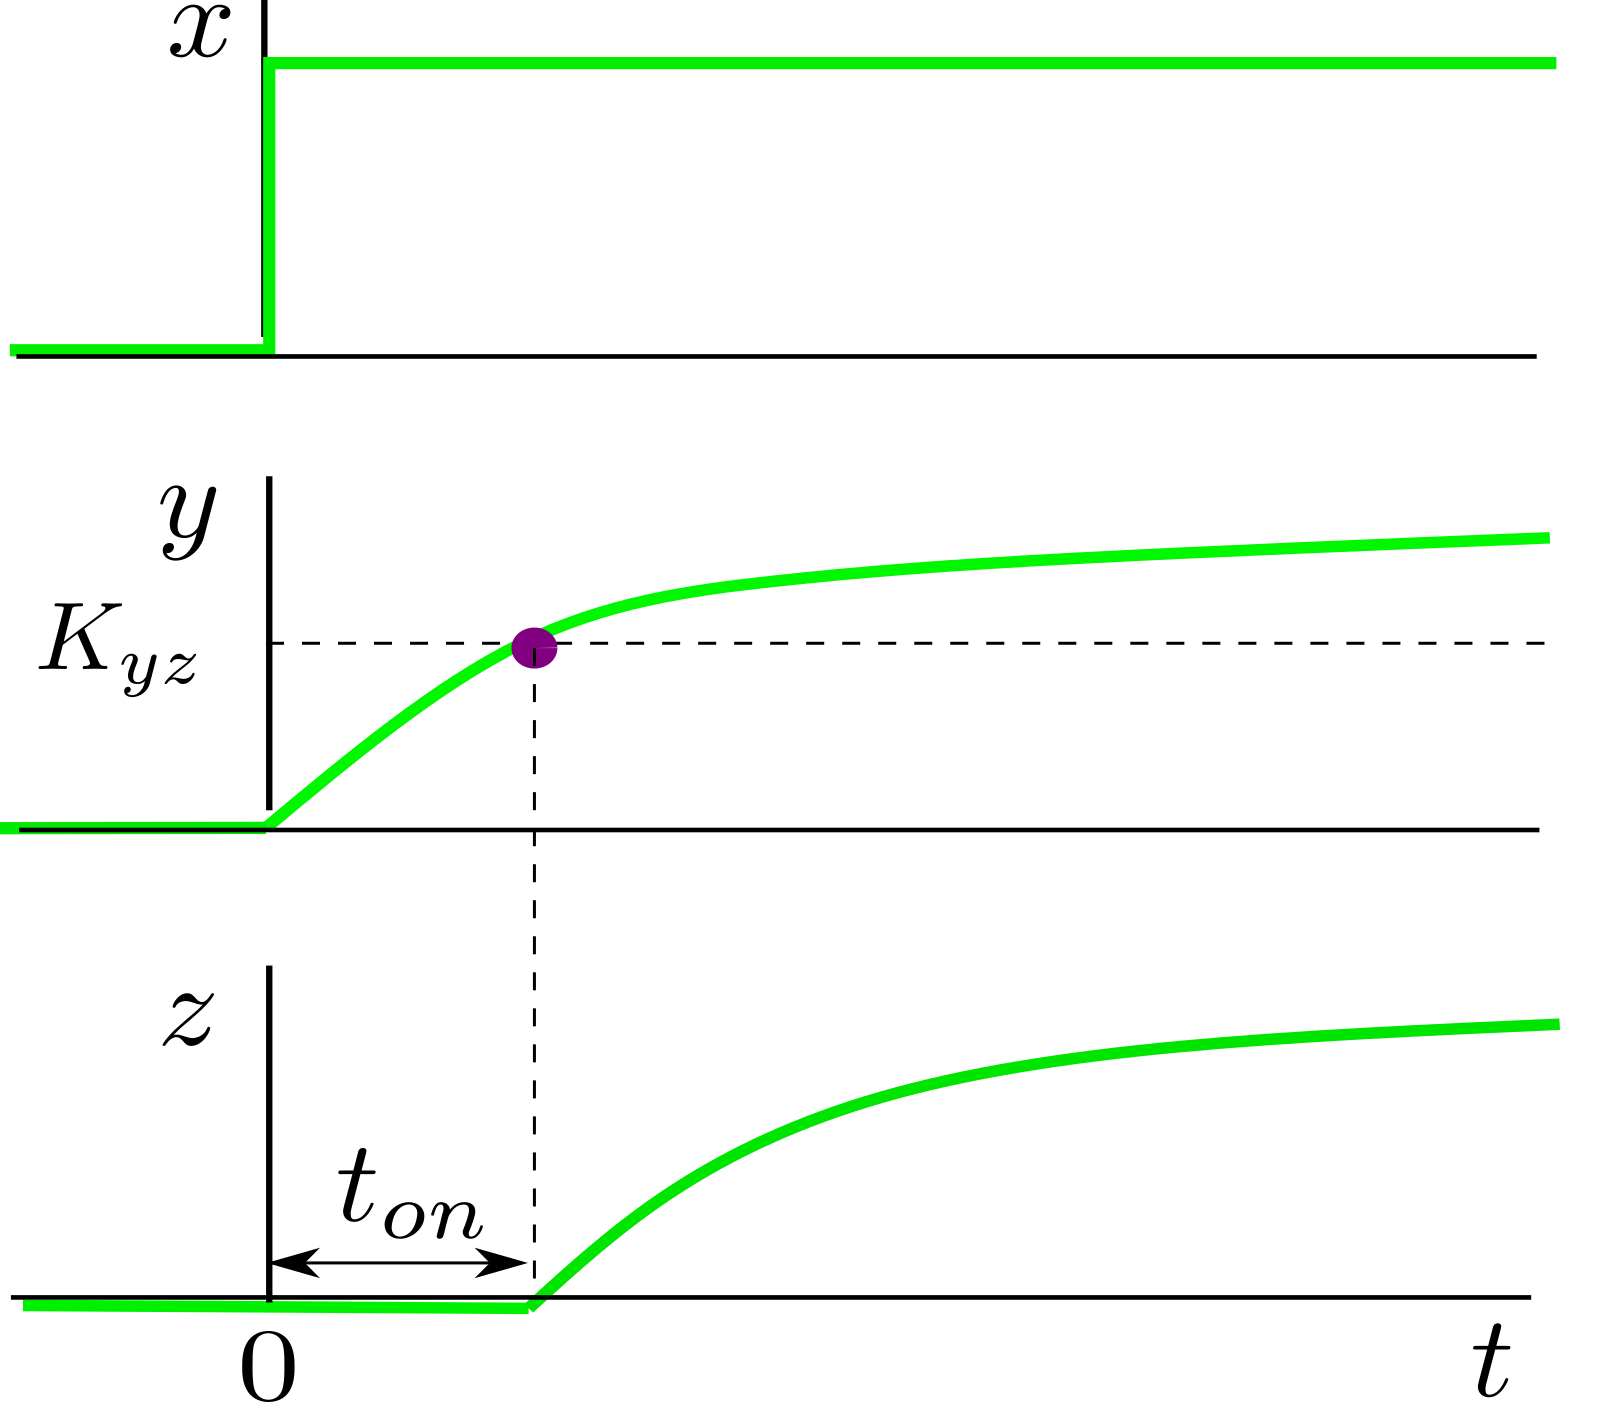
\includegraphics[height=2in]
{autoregulons/c1-ffl-up-green.png}
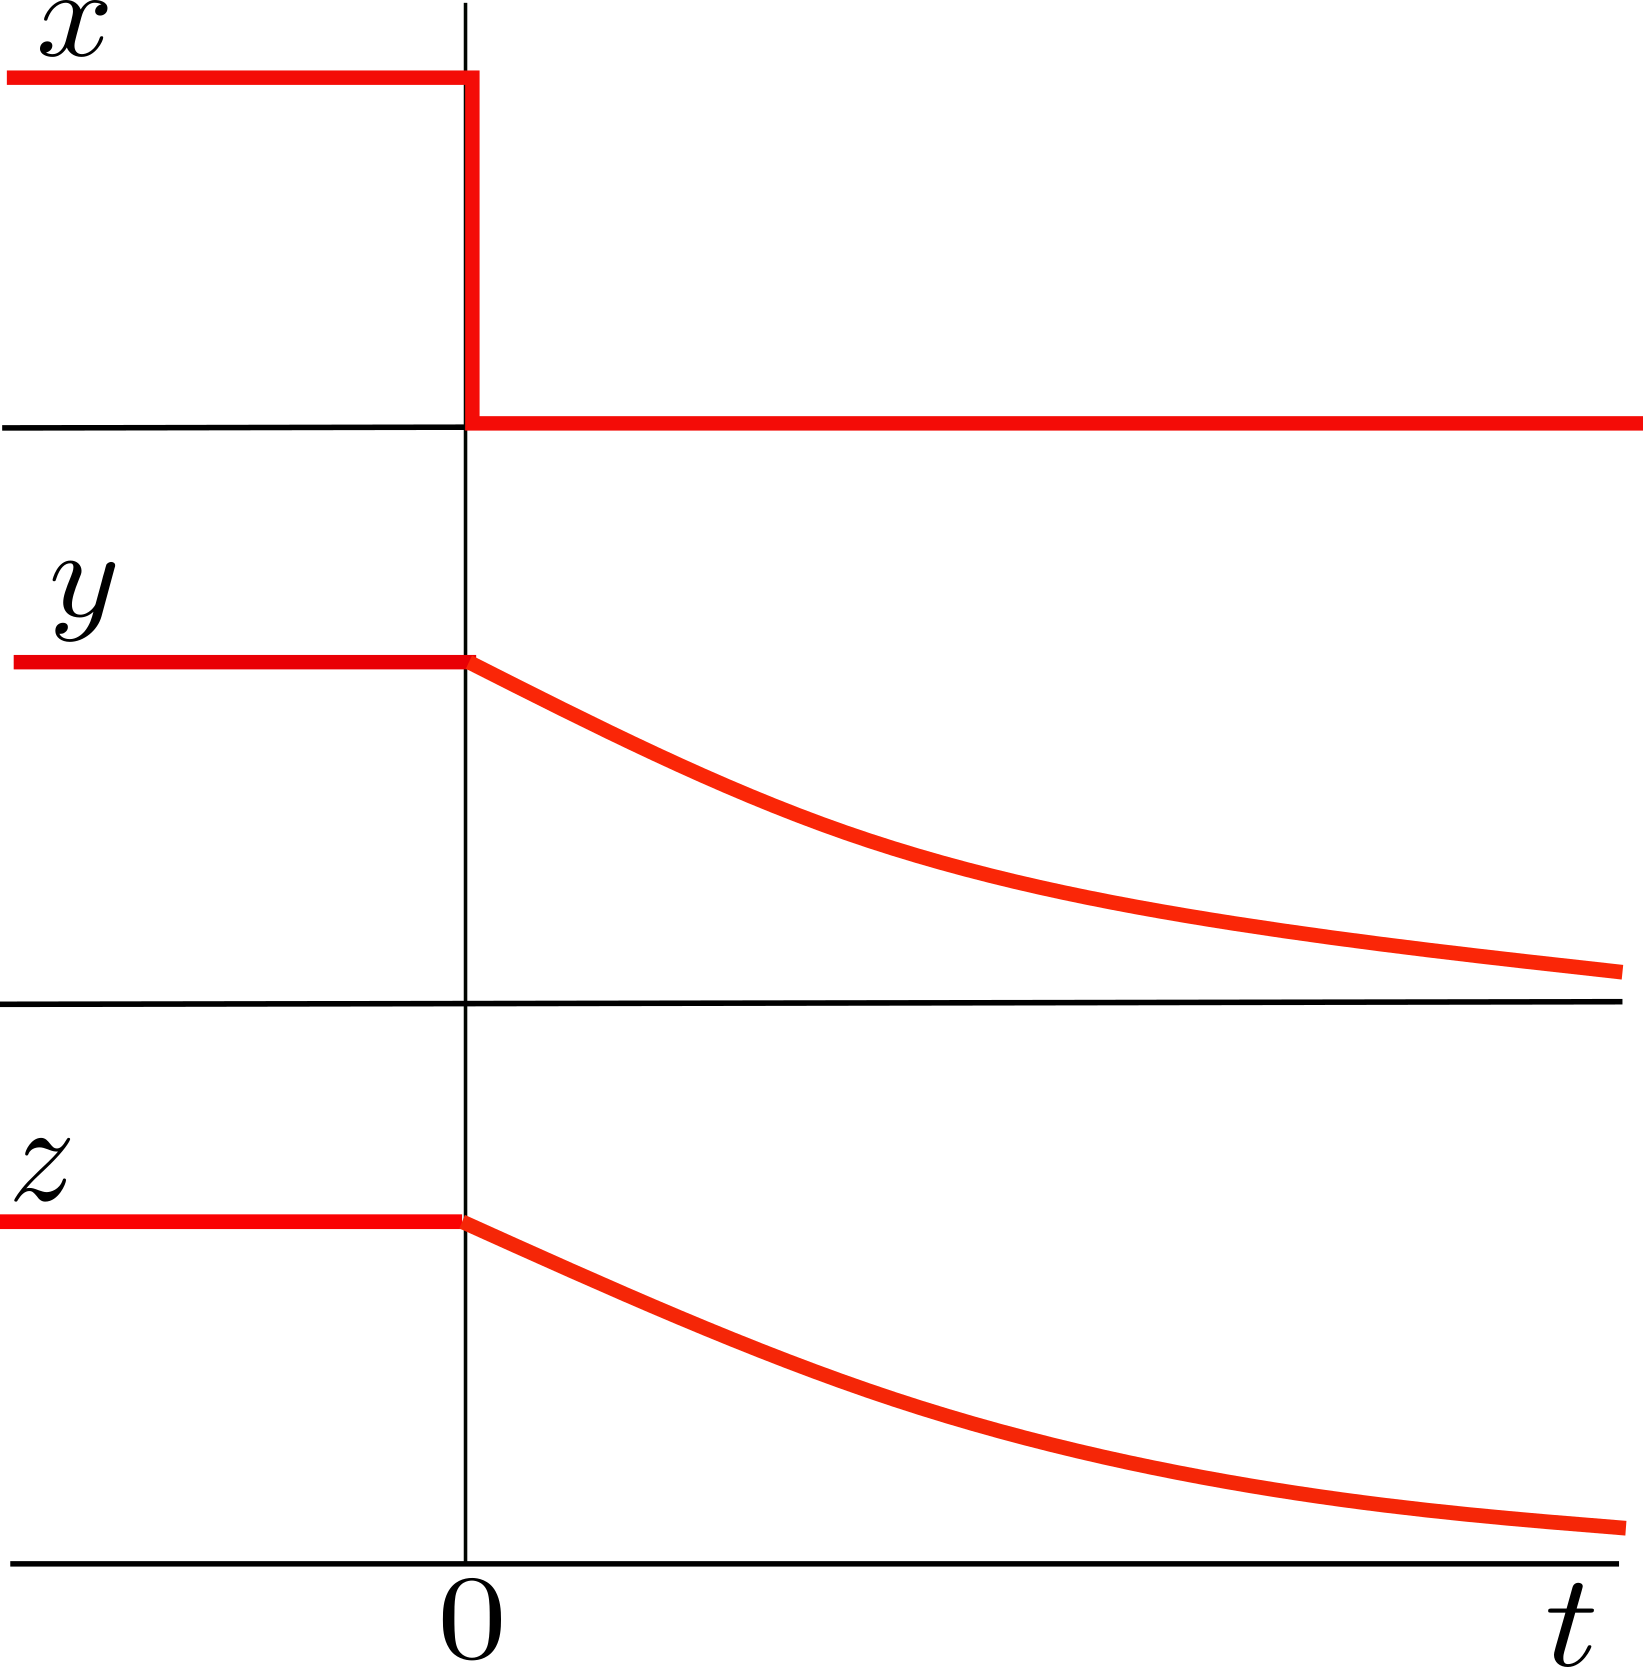
\includegraphics[height=2in]
{autoregulons/c1-ffl-down-green.png}
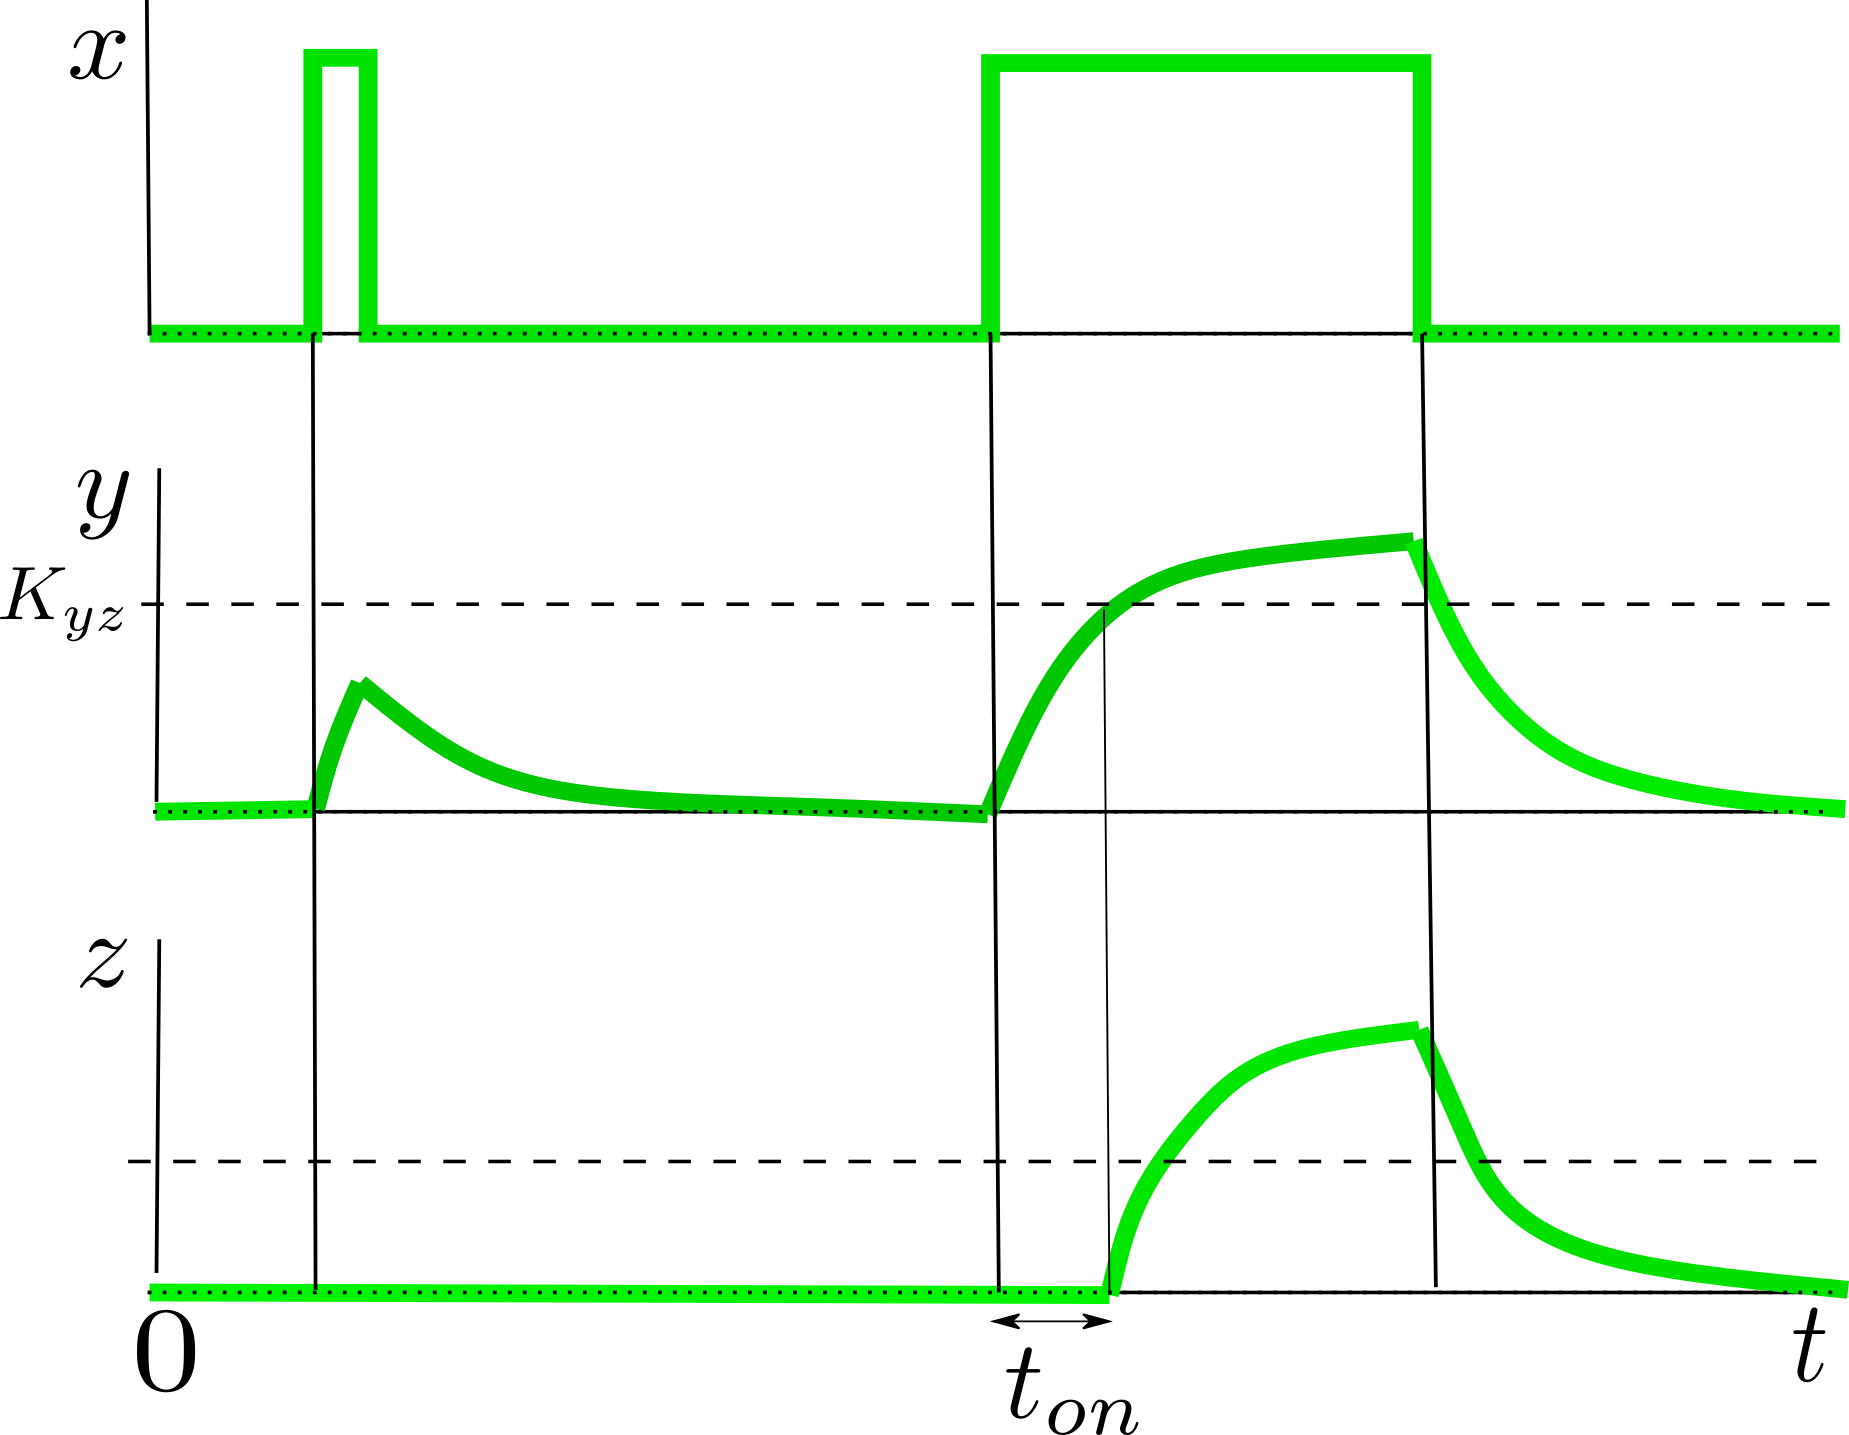
\includegraphics[height=2in]
{autoregulons/c1-ffl-up-down-green.png}
\caption{$x(t)$, $y(t)$, $z(t)$ assuming 
that $x(t)$ is either a rising step function (in green),
a dropping step function (in red),
or a square function (in purple).}
\label{fig-c1-ffl-triple}
\end{figure}



\hrule
Below, the red equations 
correspond to a different choice of $x(t)$.

Assume (see Fig.\ref{fig-c1-ffl-triple})
\beq
x = x_0\indi(t>0)
\eeq
\beq \nonumber
\color{red}
x = x_0\indi(t<0)
\eeq
where $x_0 > K_{\rvx\rvy}, K_{\rvx\rvz}$.
Thus, Eq.(\ref{eq-ffl-gen}) reduces to

\beq
\left\{
\begin{array}{l}
\dot{y} = \beta_\rvy
-\alp_\rvy y
\\
\dot{z} =  \beta_\rvz
\indi(y>K_{\rvy\rvz}) -\alp_\rvz z
\end{array}
\right.
\label{eq-ffl-red}
\eeq
Let $
y(0) = 0, y_{ss} = \frac{\beta_\rvy}{\alp_{\rvy}}
$.\
Then (see Fig.\ref{fig-c1-ffl-triple})

\beq
y = y_{ss}(1-e^{-\alp_\rvy t})
\eeq
\beq \nonumber \color{red}
y = y_0e^{-\alp_\rvy t}
\eeq
If $y_{ss}> K_{\rvy\rvz}$, then (see Fig.\ref{fig-c1-ffl-triple})


\beq
z = \frac{\beta_\rvz}{\alp_\rvz}(1- e^{-\alp_\rvz (t-t_{on})})
\eeq
\beq\nonumber
\color{red}
z = z_0 e^{-\alp_\rvz t}
\eeq
where $t_{on}$ is defined so that

\beq
y(t_{on}) = K_{\rvy\rvz}= y_{ss}(1-e^{-\alp_\rvy t})
\eeq
Solving the last equation for $t_{on}$ yields (see 
Fig.\ref{fig-minus-log-1-minus-x.png})

\beq
y_{on} = -\;\frac{1}{\alp_\rvy}
\ln
\left({1- \frac{K_{\rvy\rvz}}{y_{ss}}}
\right)
\eeq

\begin{figure}[h!]
\centering
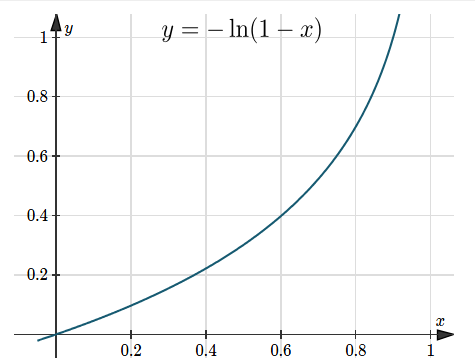
\includegraphics[width=2.8in]
{autoregulons/-log(1-x).png}
\caption{View of Mount Vesuvius from
  Pompeii.
  Picture from Ref.\cite{alon-book}.}
\label{fig-minus-log-1-minus-x.png}
\end{figure}

Fig.\ref{fig-c1-ffl-triple}
shows the waveforms for $x(t), y(t), z(t)$
assuming $x(t)$ is either 
a step function rising from 0 at $t=0$,
a step function falling to zero at $t=0$,
or a square wave rising from 0 at time $t=0$
and falling to 0 a while later.

\hrule
\begin{figure}[h!]
\centering
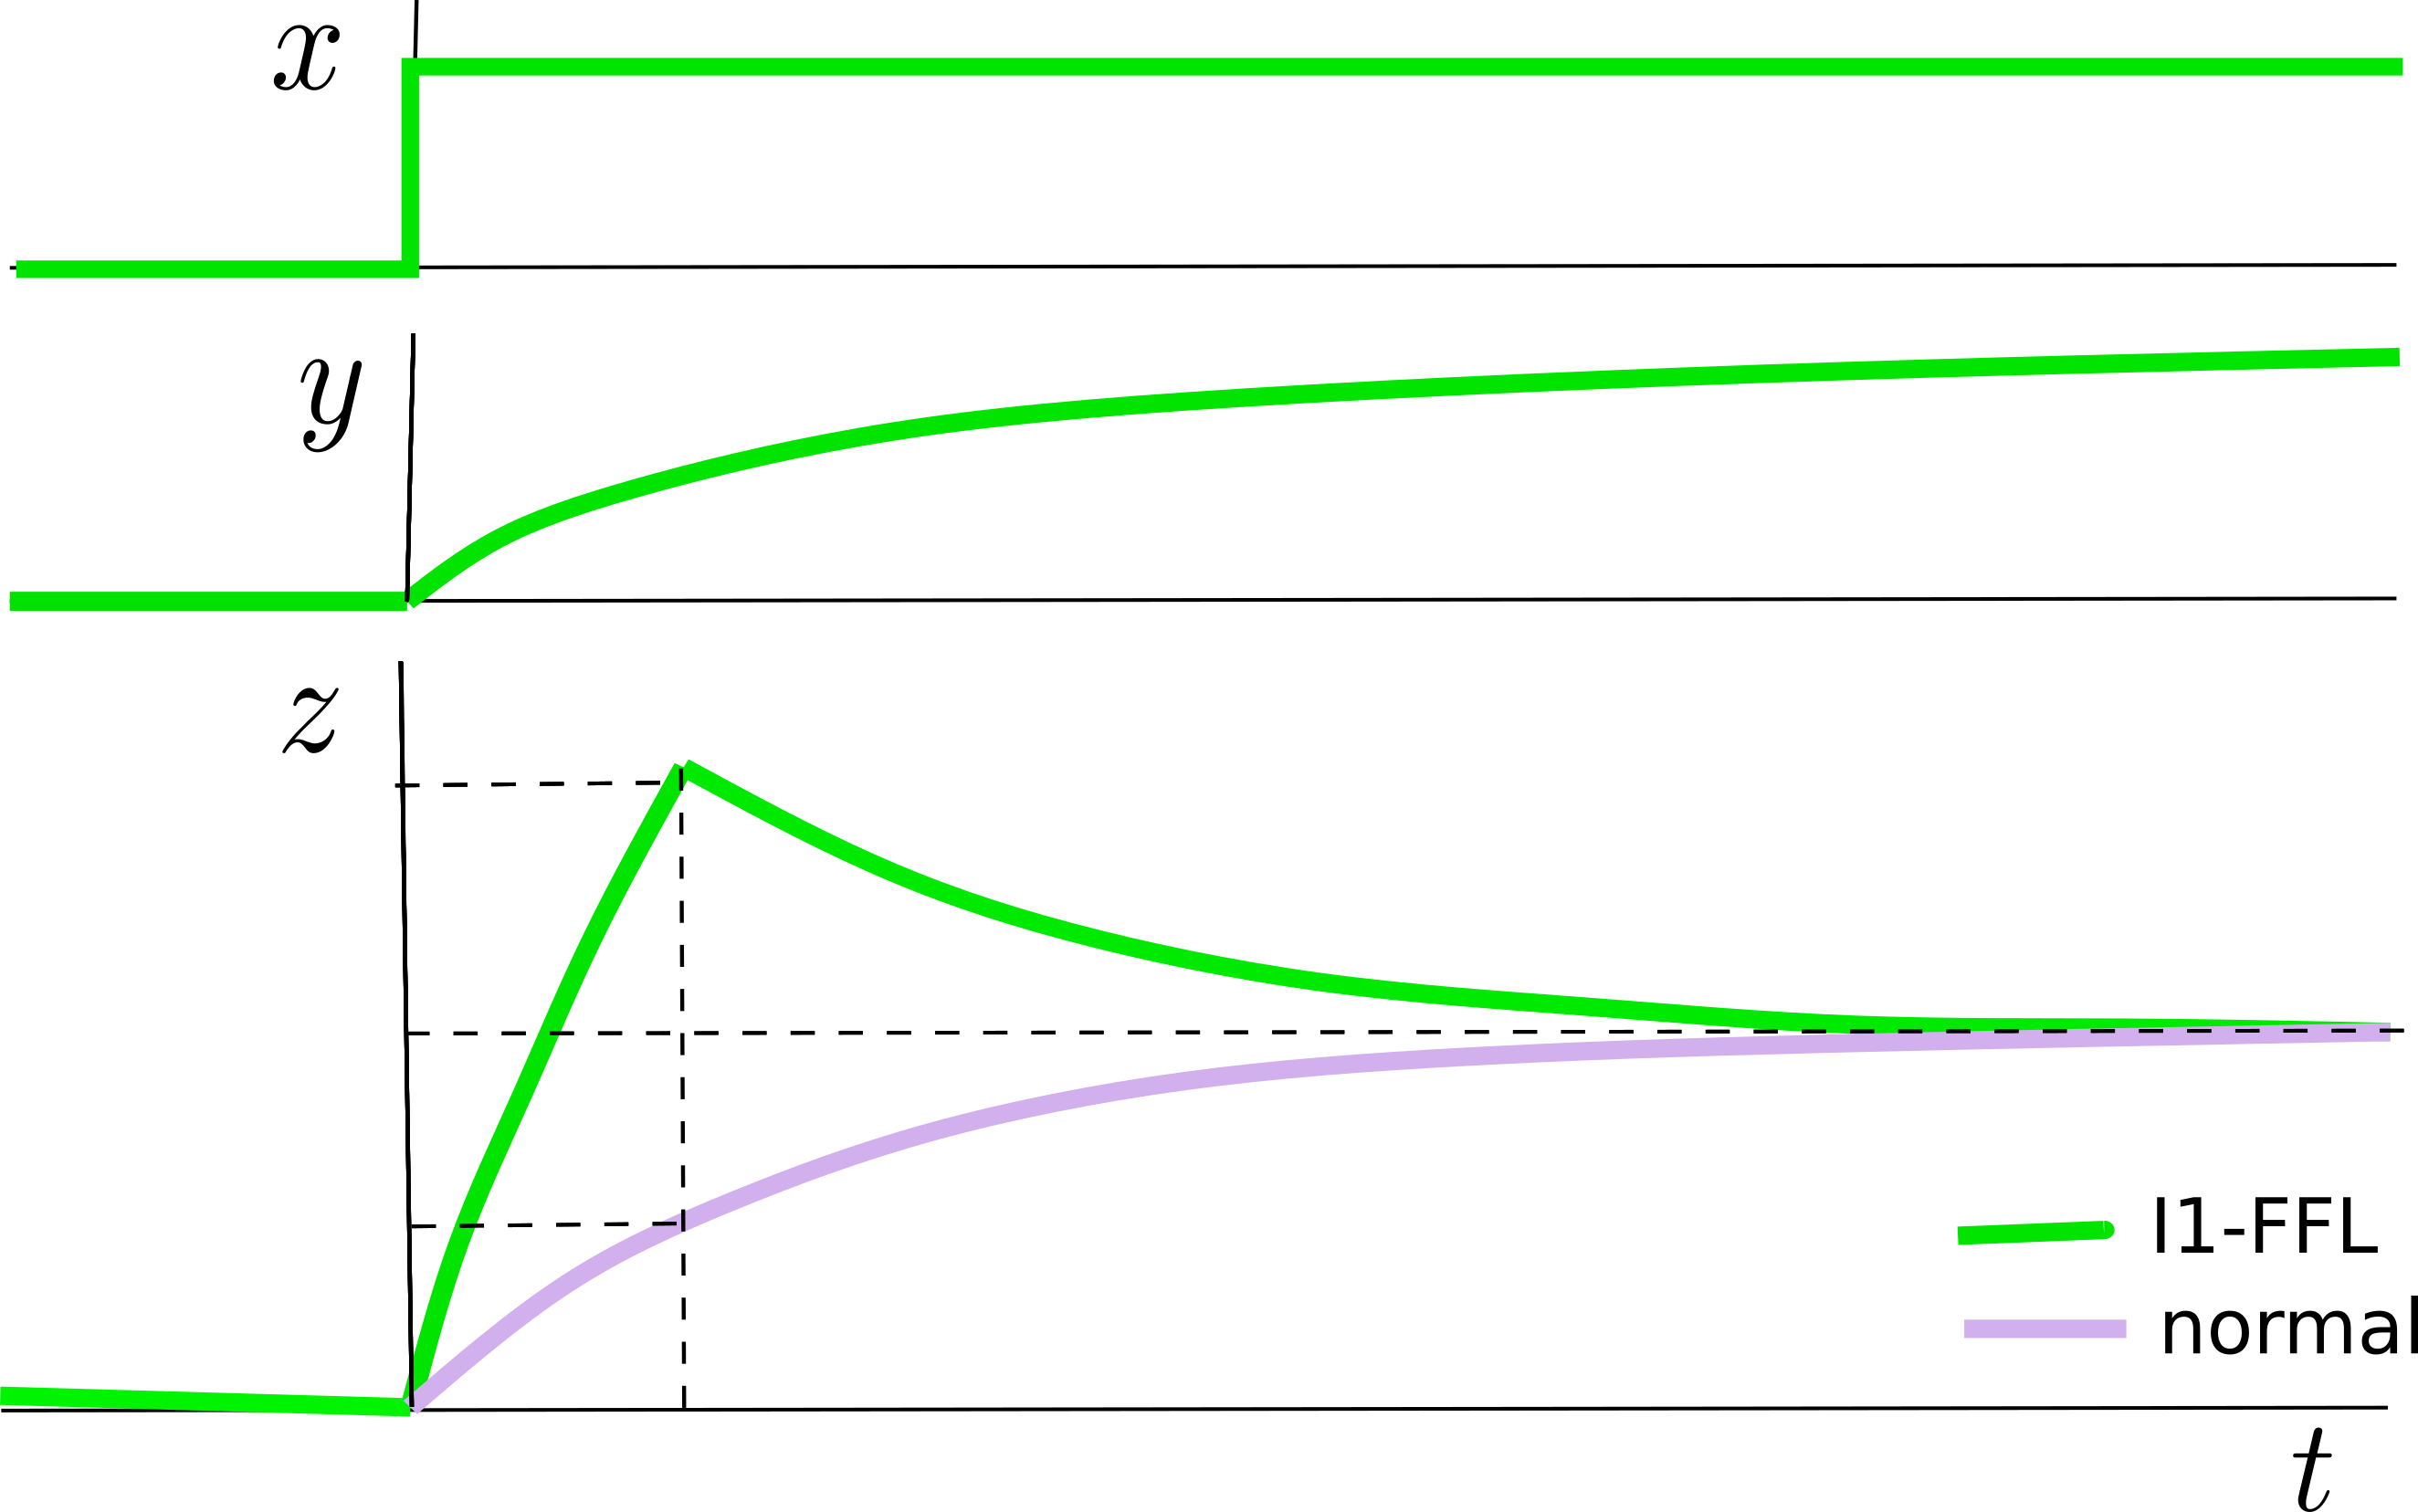
\includegraphics[width=2.8in]
{autoregulons/i1-ffl-green.png}
\caption{View of Mount Vesuvius from
  Pompeii.
  Picture from Ref.\cite{alon-book}.}
\label{fig-i1-ffl}
\end{figure}

\section{SIM net}
Single Input Module (SIM) net

\section{FFL net}

Feedforward Loop (FFL) net

\section{Bistable net}

\section{Biological clock net}